\section{The platform}

Any language can be used both as string-embedded or host language. For each combination it could be necessary to solve different tasks: from errors detection to additional information extraction and metrics computation. As there are substantial number of languages combinations and different types of tasks, our research is not aiming to create a tool that handles all possible scenarios. The main goal is to create the platform that simplifies the process of building endpoint tools for the certain languages and tasks. The similar approach can be seen in the tools for compilers development. Usually such tools include lexical and syntax generators and utility functions libraries to simplify the process of  specific compiler creating.

Being complex and self-contained task, the host language analysis is assumed to be performed by some external tool. Moreover, this tool is assumed to return a source code's AST which contains the information needed for further steps as a result of it's work.

The platform is to perform the whole process of string-embedded languages handling. It includes the following steps:
\begin{itemize}
\item dynamically generated expressions can have a set of possible values so the approximation of the set is to be constructed;
\item lexical analysis is to be applied to the FSA that has been obtained after approximation;
\item syntax analysis is to be performed resulting in the parse forest;
\item parse forest analysis and semantics calculation is to be performed.
\end{itemize}

\subsection{Architecture}

The platform's architecture is shown in Figure~\ref{platform_architecture_ref}.

\begin{figure}[h!]
    \begin{center}
        \includegraphics[scale=0.3]{Figures/SELYCcomponents.png}
    \end{center}
    \caption{The platform's architecture}
    \label{platform_architecture_ref}
\end{figure} 

The Approximation component is responsible for building the set of strings with embedded code that can be produced by the host language program. The elements of that set are to be statically analysed. This set can be considered as a language where the words are the strings with embedded code. In general the language can be recursively enumerable. Many problems are undecidable for this class of languages that makes it hard to work with. One possible solution is to build an upper regular approximation of the language we have. In other words we build the regular language that contains all the words of the language we have and, possibly, some other words. It is important to note that the regular language must be as close as possible to the language it approximates. It means the language must keep the number of "extra" words to a minimum. Despite the fact we end up with the approximation of the initial set, working with a regular language makes the further analysis much easier. Moreover, regular languages can always be represented as FSA that is convenient to manipulate.

The Approximation component accepts a generalized CFG with some additional information as an input. As an output it produces the FSA that encodes the approximated set of strings with embedded code.

The lexing component consist of two parts. The first one is the lexer's generator which generates finite-state transducer(FST,~~\cite{FST:ref}) from the provided lexical specification of the string-embedded-language. The second one is the interpreter which analyzes the data structure passed using generated FST. The lexing component accepts FSA over symbols alphabet and produces the FSA over alphabet of processed language tokens.

The parser generator is based on the RNGLR algorithm~\cite{RNGLR:ref}. Using the grammar of the language processed the generator builds parse tables. Then the analyzer, which is implemented as a separate library, parses the FSA that was obtained after the lexical analysis. The result is a shared packed parse forest (SPPF~\cite{SPPF:ref}) which is a compact structure that allows to reuse common nodes along different ASTs. This structure can be used for the further processing: for additional information extraction or to implement such IDE functionality as "go to definition".

\subsection{Approximation}

The process of building the set of strings with embedded code can be divided into two steps:
\begin{itemize}
\item finding the string expressions with embedded code in the source code;
\item building the set of possible values for found string expressions.
\end{itemize}

The first step is not implemented in our platform. This functionality is assumed to be implemented by the platform's user. The second step is performed by the platform and described in more detail below.

\subsubsection{Upper regular approximation building}

This section briefly describes the regular approximation building algorithm, presented in~\cite{Upper_Approximation:ref}. The paper~\cite{Upper_Approximation:ref} is devoted to the analysis of string expressions produced by PHP code. The analysis is aimed to find the expressions that can be used to perform malicious actions. We are interested in the algorithm presented because it guarantees building the upper approximation. Moreover, it handles most host language operations that can be used to form string expressions.

To begin with we introduce some definitions. \textit{Target expression} -- the string expression in the source code which possible values are to be built. \textit{Target node} -- the node in the control flow graph (CFG) containing target expression. \textit{Data-dependency graph (DDG)} -- directed graph that represents dependencies between instructions in the source code. Graph nodes correspond to expressions in the source code. The edge from the node \verb|X| to the node \verb|Y| indicates we need to calculate the expression in the node \verb|X| before we can calculate the expression in the node \verb|Y|.

As an example consider Listing ~\ref{code_fragment} where the reference to the \verb|"sql"| variable in the line 10 is chosen to be the target expression. Figure~\ref{flow_graph_pic} shows the CFG for the code fragment from the listing where the node 16 is a target node. DDG for the \verb|"sql"| reference is shown in Figure~\ref{data_dependency_pic}.

\begin{lstlisting}[label=code_fragment,caption=C\# code fragment]
Entries GetEntries(boolean cond) 
{
    string logMsg = "Selected";
    string sql = "SELECT * FROM ";
    if(cond)
      sql = sql + "Table1";
    else
      sql = sql + "Table2";
    Console.WriteLine(logMsg);
    return Db.Execute(sql);
}
\end{lstlisting}


\begin{figure}[h!]
    \begin{center}
        \includegraphics[scale=0.3]{Figures/Flow_graph.png}
    \end{center}
    \caption{Control flow graph for the code fragment from the Listing~\ref{code_fragment}}
    \label{flow_graph_pic}
\end{figure} 


\begin{figure}[h!]
    \begin{center}
        \includegraphics[scale=0.3]{Figures/Dependency_graph.png}
    \end{center}
    \caption{Data-dependency graph for the \texttt{"sql"} variable reference from the Listing~\ref{code_fragment}}
    \label{data_dependency_pic}
\end{figure} 

Further the following agreement about finite-state automata will be used. It is assumed every automaton has an additional state that is not shown explicitly. This state is called a sink state. The sink state is not a final one and transitions for all symbols of the automaton's alphabet lead to the sink state itself. When some automaton is mentioned in the text or illustrated in a picture transitions will be defined only for some symbols of the alphabet. It is assumed that if the transition for the symbol  \verb|'a'| from the state \verb|X| is not defined explicitly it leads to the sink state (see Figure~\ref{hi_pic}). Sink states are omitted for simplicity.

\begin{figure}[h!]
    \begin{center}
        \includegraphics[scale=0.3]{Figures/automaton_with_sink.png}
    \end{center}
    \caption{Simplified illustration of the automaton over the alphabet A (1) and corresponding fully determined one with sink state (2)}
    \label{hi_pic}
\end{figure} 

Now we describe the regular approximation building algorithm presented in~\cite{Upper_Approximation:ref}. It consists of the following steps:
\begin{itemize}
\item control flow graph is created for the source code;
\item based on the CFG and some target node in it the data-dependency graph is computed;
\item finite state automata are constructed for the expressions in the DDG nodes. Automata are the upper approximations of the expressions' possible values sets. Automaton corresponding to the target node is returned as a result.
\end{itemize}

Let us see how exactly automata are built for the expressions in the nodes during the DDG traversal.

{\bf String literals.} The FSA for the string literal is an automaton that accepts only this literal. The example for the literal \verb|"hi"| is shown in Figure~\ref{hi_pic}.

\textbf{Strings concatenation.} The concatenation operation is performed on two automata that correspond to the operation arguments. Based on these automata the resulting one is built. It accepts the strings that consist of prefix and suffix. The prefix is any string accepted by the first argument automaton and the suffix is any word accepted by the second argument automaton (see Figure ~\ref{concat_pic}).

\begin{figure}[h!]
    \begin{center}
        \includegraphics[scale=0.3]{Figures/automata_concat.png}
    \end{center}
    \caption{Argument automata (1) and their concatenation (2)}
    \label{concat_pic}
\end{figure} 

\textbf{Replace in strings.} Replace operation expects three automata as the arguments (see Figure~\ref{replace_pic}). The first one contains strings where the replace must be performed (Figure~\ref{replace_pic}(1)). The second one contains strings to be searched as substrings in the strings of the first automaton (Figure~\ref{replace_pic}(2)). The third one encodes the set of strings to be used as a replacement(Figure~\ref{replace_pic}(3)).

\begin{figure}[h!]
    \begin{center}
        \includegraphics[scale=0.3]{Figures/automata_replace.png}
    \end{center}
    \caption{Replace operation arguments (1), (2) and (3) and the operation result (4)}
    \label{replace_pic}
\end{figure} 

\textbf{Conditional expressions (if, if-else).} Suppose there is node \verb|A| in the DDG. If the expression in the node \verb|A| depends on some expression that can be constructed in different branches of the conditional operator there are several (two in case of if-else) paths leading to the node \verb|A|. Same type expressions are constructed along all these paths. To collect the information about all these possible expressions one must union all the automata obtained after traversing each path leading to the node \verb|A|.

\textbf{Loops.} Loops processing is challenging. Firstly, during the static analysis it is often impossible to define how much iterations of the loop will be executed. So in general the loop produces an infinite language. Secondly, the language can be non regular and the example of such a case is shown on Listing~\ref{classic_example}. The fragment generates strings from the set $\{ a^nb^n |\; n = 1,\; 2 \ldots \}$, that is a classic example of a nonregular language.

\begin{lstlisting}[label=classic_example,caption=Loop with a replace operation in C\#]
String str = "ab";
for(...) {
  str = str.Replace ("ab", "aabb");
 }     	
Db.Execute(str);
\end{lstlisting}

To overcome the problems described the widening operator is used. The operator accepts two automata as the arguments and defines a special equivalence relation on the set of their states united. The equivalence classes formed by this equivalence relation are used as states for the resulting automaton, transitions are created based on the transitions of the argument automata. This resulting widened automaton accepts all the words accepted by the argument automata and generalizes these automata in some sense.

The operator is used for two automata that are the results of two successive loop iterations as follows:
$$
A_i' \;=\; \nabla (A_i \cup A_{i-1}, A_{i-1})
$$

where $A_i$, $A_{i-1}$ -- are the automata generated after current and previous iterations respectively, $\nabla$ -- widening operator. The $A_i'$ automaton is used as a new result of the current iteration. What is important is that the sequence $A'_i$, $i \;=\; 1, 2 \ldots$ is always converge~\cite{Upper_Approximation:ref}, i.e. beginning from some $m$:
$$
\forall i > m \colon A'_i \;=\; A'_{i+1} \;=\; R
$$

The notation  $A'_i \;=\; A'_{i+1}$ means the automata are equivalent, i.e. they define the same regular language. The automaton $R$ is set to be the result of the loop's approximation. In fact, here we solve the least fixed point computation problem.

Let us consider the example of widening operator usage for the loop in the Listing~\ref{example_loop}. The process of automata construction is presented in Figure~\ref{automata_loop_pic}. For each iteration the following automata are shown: the initial one -- constructed as a result of loop body processing; the united automaton -- constructed as a union operation result of the initial automaton and the automaton obtained in the previous iteration; the widened automaton -- constructed as a result of applying widening operator to the united automaton and  the automaton obtained in the previous iteration. If there is a dashed arrow from the automaton \verb|A| to automaton \verb|C| and from \verb|B| to \verb|C| the \verb|C| is constructed from \verb|A| and \verb|B| using the operation which name is written in the same line the automaton \verb|C| is placed (for example, union operation).

\begin{lstlisting}[label=example_loop,caption=Loop with concatenation on C\#]
String str = "a";
for(...) {
  str += "b";
}     	
Db.Execute(str);
\end{lstlisting}

It can be seen from the example the sequence of widened automata is converge on the third iteration. That is the widened automaton of the third iteration, accepting words from the set $\{ ab^{*} \}$, is set to be the approximation result of the loop from the Listing~\ref{example_loop}.

\begin{figure}[h!]
    \begin{center}
        \includegraphics[scale=0.3]{Figures/automata_loop.png}
    \end{center}
    \caption{Approximation building for the loop from Listing~\ref{example_loop}}
    \label{automata_loop_pic}
\end{figure} 

\textbf{User input functions.} User input functions like reading from a console or file can return any strings and it is impossible to predict these strings values during the static analysis. Therefore, it is assumed the automaton for the return values of such functions is an automaton accepting any words.

Formal definitions of concatenation, replace and widening operations for the FSA are given in~\cite{Upper_Approximation:ref}.

Let us consider the example of FSA building for the DDG in Figure~\ref{data_dependency_pic}. The following steps will be performed.
\begin{enumerate}
\item Nodes 1, 2 and 3 contain literals, so for each of them the FSA accepting corresponding literal will be constructed.
\item After node 4 is processed the FSA constructed for node 2 will be bound to the name \verb|"sql"|.
\item For node 7 the automaton will be constructed which is the result of concatenation of the automaton named \verb|"sql"| and the automaton from node 1. The same is for node 8 but the second argument of the concatenation is obtained from node 3. The resulting automaton for node 7 will accept the literal  \texttt{"SELECT * FROM Table1"} and the automaton for node 8 -- literal \texttt{"SELECT * FROM Table2"}.
\item In nodes 9 and 10 the automata from nodes 7 and 8 respectively will be bound to name \verb|"sql"|.
\item The final node 11 is a node where alternative branches of conditional operator are merged. So the automata with the same names obtained from the alternative branches will be united here. That is, the resulting automaton for node 11 is the one that accepts both literals \texttt{"SELECT * FROM Table1"} and \texttt{"SELECT * FROM Table2"}.

\end{enumerate}

\subsubsection{Implementation details of the approximation algorithm}

One should note the implementation details of the described algorithm in our platform.

On the first step of the algorithm we create so called generalized CFG instead the usual one. The generalized CFG has the same structure as the usual one, but instructions in nodes are replaced with abstract ones. So in fact the generalized version represents the control flow of a pseudocode of the initial program. It is assumed that to build the approximation for some specific language one should convert language specific CFG to general one. This makes the platform able to support multiple host languages.

The approximation is built for some function (or method) where the strings with embedded code are constructed. During the processing of this function, the ones called from it are processed too. So the interprocedural approximation is built. To process the function calls the whole approximation algorithm is repeated recursively with the called function's return statement being a target expression. The recursion depth is constrained by some number that is defined as the algorithm's parameter and can be changed if needed. If the recursion depth becomes equal to the constraining parameter value the subsequent function calls are not processed anymore. The FSA accepting any words is used as the approximation result of this subsequent function calls.

The function called in source code under processing can be recursive itself. In this case the algorithm will always achieve constrained recursion depth and the approximation will be inaccurate because the FSA accepting any words will be used. In the case when called function is tail recursive we overcome described problem with special preprocessing. The generalized control flow subgraph  corresponding to tail recursive function call is replaced with the subgraph corresponding to the loop equivalent to this tail recursive function. This loop is processed then with widening operator as any other loop. For non tail recursive functions there is no special treatment for now.
\subsection{Lexical and syntax analysis}

The purpose of the lexical analysis is to extract tokens defined by the language specification from the input stream of symbols. Also the correspondence between lexical units and the source code must be preserved. The result of lexical analysis of the dynamically generated expression is a finite-state automaton over the alphabet of tokens. In the classic lexical analysis the token can be represented by some identifier and the subsequence of input symbols. In the case of dynamically generated expressions analysis the input symbols subsequence is replaced by the FSA representing the subset of all possible values of dynamically generated expression. Moreover, in the latter case for each symbol we must preserve the information about its position in the source code.

Lexical analysis consists of four steps. Firstly, the input FSA that was build by the approximator is transformed into the deterministic one. After that the FST is constructed based on the FSA. The next step is to build the composition of the obtained FST and the FST that was built based on the language specification. This second FST produces tokens as an output. The composition is a result of the consecutive application of these two transducers, i.e. an output of first FST is used as an input for the second. After that we obtain either a set of lexical errors or a FST with a pair on each edge. The first item in the pair is the symbol with the binding to the source code, the second one is a function that returns either token or nothing. If the previous step end up with no errors, the last step is an interpretation of the FST resulting in a finite-state automaton over the tokens alphabet.

This automaton is processed by the syntax analyzer. The analyzer is based on RNGLR~\cite{RNGLR:ref} algorithm which is a modification of Tomita's GLR-algorithm\cite{Tomita:ref}. Tomita's GLR algorithm allows to handle arbitrary context-free grammars. GLR handles Shift/Reduce and Reduce/Reduce conflicts -- situations when an available data are not enough to choose the correct way of parsing. Therefore, GLR processes all possible ways in case of conflict. So several derivation trees for a single input sequence can be obtained. The parser used in our platform extends this approach. The algorithm processes a token graph as an input. Herewith we meet a new situation when one node has several outgoing edges. We call this a "Shift/Shift" conflict despite the fact it is not an actual conflict because each way should be processed. More detail about the parser algorithm can be found in~\cite{AGLR:ref}. 
\subsection{SPPF analysis and semantics calculation}

The result of dynamically generated expressions parsing is a parse forest represented by the structure called SPPF~\cite{SPPF:ref}. This structure allows to reuse common subtrees for different trees.

Based on SPPF it is possible to build a so called compound control flow graph and try to solve classic static analysis tasks using it. When building compound CFG we assume that the string-embedded language grammar is a grammar of some programming language and that a mapping between non-terminals and CFG blocks is defined. For instance the \verb|"if_stmt"| non-terminal derivation should be treated as the conditional block in CFG. Other example is shown in Figure~\ref{simple_example_pic}, where the \verb|"assignment"| non-terminal derivation is treated as the assignment operation in CFG.

\begin{figure}[h!]
  \begin{center}
    \begin{subfigure}{0.3\textwidth}    
        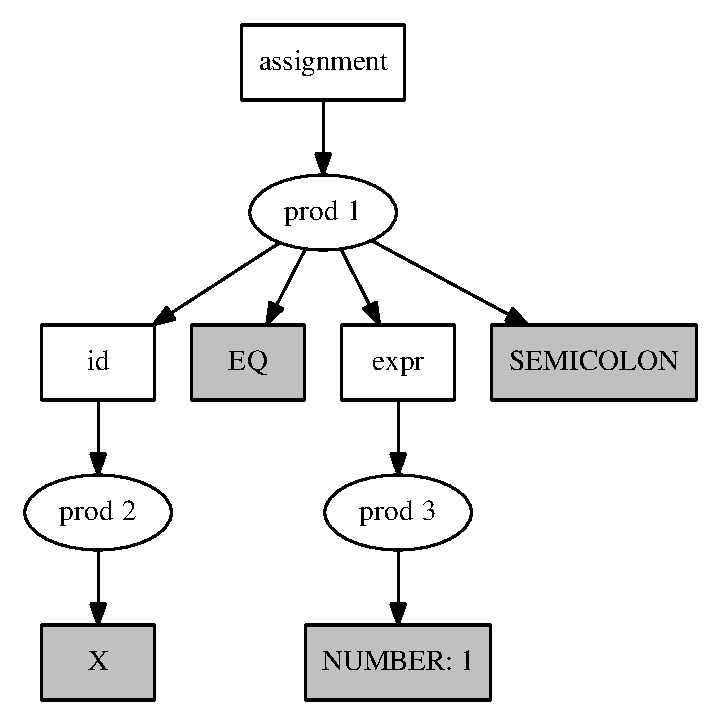
\includegraphics[scale=0.3]{Graphs/cfg_idea.eps}    
    \caption{}
    \label{simple_a}
    \end{subfigure}
    \begin{subfigure}{0.1\textwidth}      
            \includegraphics[scale=0.5]{Graphs/assignment_simple.eps}        
     \caption{}
     \label{simple_b}
    \end{subfigure}
    \caption{\texttt{assignment} non-terminal derivation (\ref{simple_a}) and corresponding CFG block (\ref{simple_b})}
    \label{simple_example_pic}
  \end{center}
\end{figure}

Because of the fact that SPPF can contain several trees, the compound CFG can contain several usual CFGs. To make this possible an intermediate nodes are introduced. Further intermediate nodes will be called \textit{"nodes"} (in figures they will have oval shape) and CFG elements will be called \textit{"blocks"} (in the figures they will have rectangle shape). The derivation of \verb|"assignment"| non-terminal corresponding to sequences \verb|"X = 1;"| and \verb|"Y = 1;"| is shown in Figure~\ref{complicated_example_pic}. 

\begin{figure}[h!]
    \begin{center}
    \begin{subfigure}{0.3\textwidth}    
        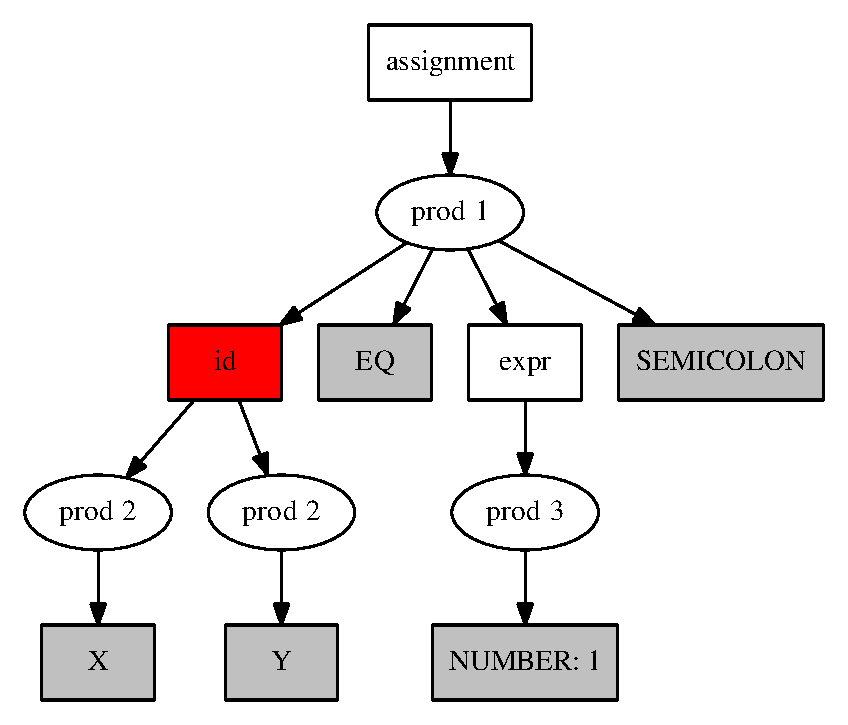
\includegraphics[scale=0.3]{Graphs/cfg_idea_complicated.eps}    
    \caption{}
    \label{complicated_a}
    \end{subfigure}
    \begin{subfigure}{0.1\textwidth}      
            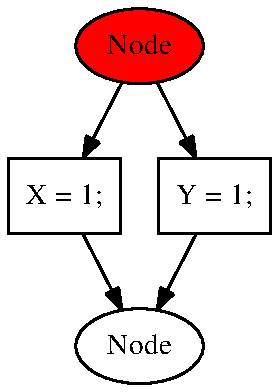
\includegraphics[scale=0.5]{Graphs/assignment_complicated.eps}
        \caption{}
        \label{complicated_b}
    \end{subfigure}
    \caption{\texttt{"assignment"} non-terminal derivation (\ref{complicated_a}) and corresponding CFG blocks (\ref{complicated_b})}
    \label{complicated_example_pic}
    \end{center}
\end{figure}
Using obtained compound CFG one can solve the static analysis tasks. Consider definite assignment analysis as an example. Here we suppose that variable is defined in the statement $\alpha$ if and only if there is a variable definition along each of the evaluation paths from the program's start to the $\alpha$ statement. 

For each block $\alpha$ the following transitions are valid:
$$
before (\alpha) \;=\; \bigcap_{\beta \;\in\; pred(\alpha)} \;after(\beta)
$$
$$
after (\alpha) \;=\; before(\alpha) \cup gen(\alpha)
$$
where
\begin{itemize}
\item $before(\alpha)$ set contains variables defined before the statement $\alpha$;
\item $after(\alpha)$ set contains variables defined after the statement $\alpha$;
\item $gen(\alpha)$ set is empty if $\alpha$ is not an assignment block and contains left-hand operand of the assignment otherwise. 
\end{itemize}

As in case of usual CFG, the algorithm traverses the graph beginning from the start node for which the empty set is associated with. The only difference is that the $pred(\alpha)$ set contains nodes, not CFG blocks. But it is easy to define the required sets:
$$
before (\beta) \;=\; \bigcap_{\alpha \;\in\; pred(\beta)} \;after(\alpha)
$$
$$
after (\beta) \;=\; before (\beta)
$$
The compound CFG is shown in Figure~\ref{cfg_example}. In the red colored node only variable \verb|X| is defined. This node have two child blocks and the list containing variable \verb|X| is passed to each block. The \verb|"Y = X + 2;"| block adds the variable \verb|Y| to the list (because \verb|Y| is defined in this block), and the \verb|"Z = X * 3;"| block adds the variable \verb|Z|. These two blocks have the same child node, therefore the intersection of parents' lists is associated with it, i.e. the list containing the only variable \verb|X|. The list is passed when the block \verb|"X = Y * Z;"| is processed. Since passed list does not contain \verb|Y| and \verb|Z|, they will be reported as undefined variables.
\begin{figure}[h!]
    \begin{center}
        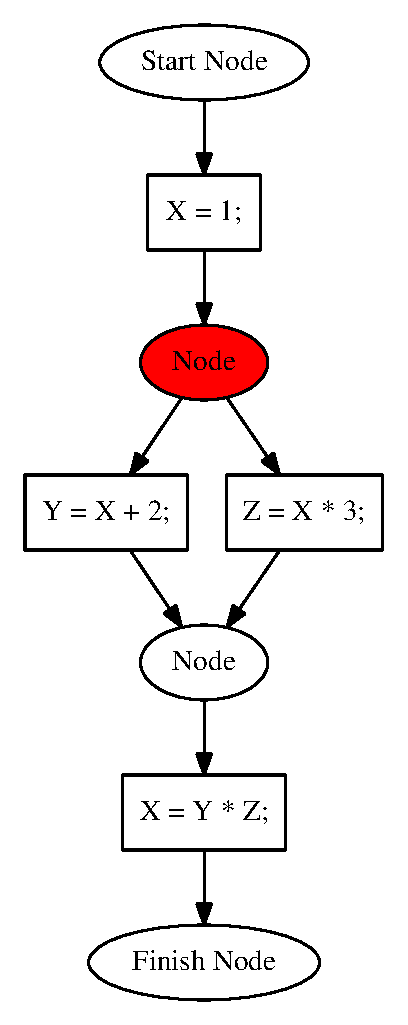
\includegraphics[scale=0.4]{Graphs/cfg_example.eps}
    \end{center}
    \caption{Compound control flow graph}
    \label{cfg_example}
\end{figure} 
